\chapter{Functional schema}

% sezione velocemente descrittiva del datapath
\section{Datapath}

% schema del datapath, possibilmente numerato 
\begin{figure}[ht]
	\centering
	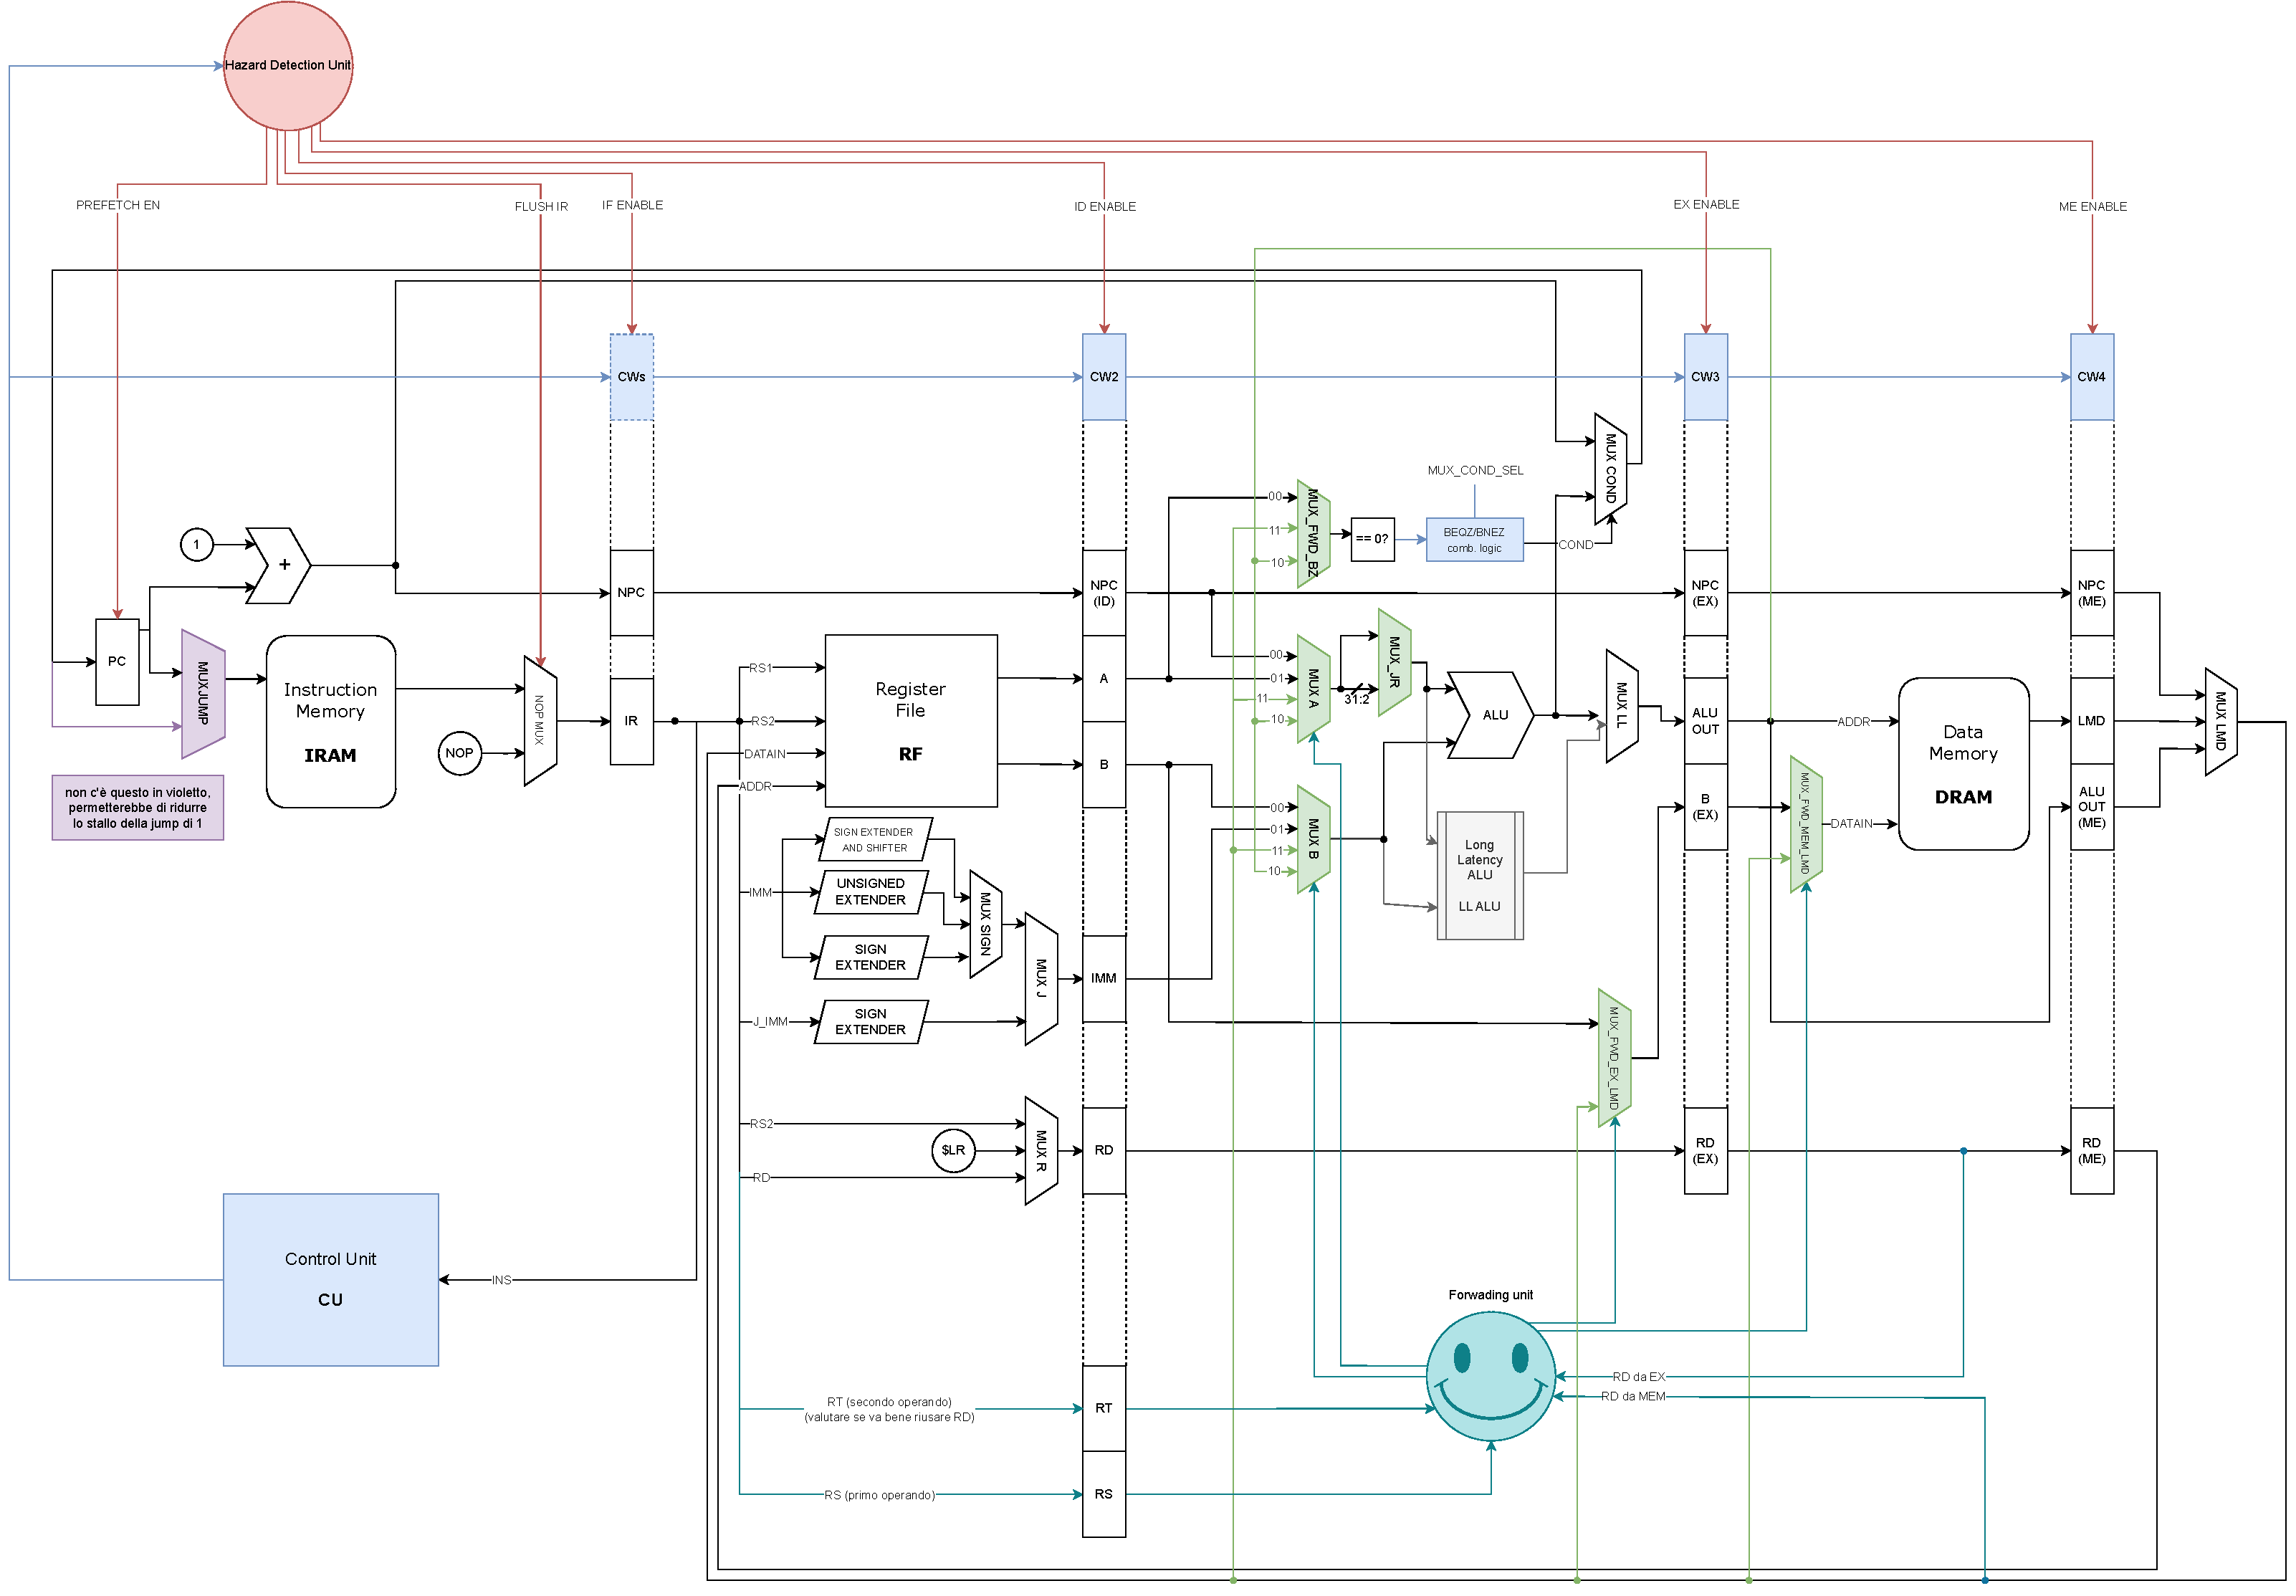
\includegraphics[width=\textwidth]{chapters/figures/datapath.pdf} 
	\caption{sus}
	\label{fig:datapath}
\end{figure}


% sezione sulle singole unità funzionali del datapath, presentate come blackbox e successivamente con l'implementazione interna, questo per ognuna di esse
\section{Functional blocks}
\subsection{Control unit}
\subsection{Register file}
\subsection{ALU}
% TODO aggiungere schema a blocchi dell'ALU
% scrivi anche come sono mussati gli ingressi
The ALU of the DLX operates on two inputs: \emph{DATA1} and \emph{DATA2}.
% la grandezza è configurabile ma è settata di default a 32 bits IIRC
% gli input muxati possono essere non solo i registri di ingresso A e B ma anche forwardati da altri stage, essere un immediato etc.
The function to be computed on the operands is selected by a third input \emph{FUNC} that receives a code representing it and the result is sent to the output \emph{OUTALU}. A list of currently implemented functions follows. The implementation of each operation is behavioural unless specified otherwise. 

% TODO fix indentations
\subsubsection{Addition}
$ \mathit{ALUOUT} = \mathit{DATA1} + \mathit{DATA2} $

A P4 adder is present inside the ALU to perform additions. Further details on its implementation together with the VHDL description are included in lab 2's zip file.

\subsubsection{Subtraction}
$ \mathit{ALUOUT} = \mathit{DATA1} - \mathit{DATA2} $


The P4 adder is also used for subtractions, by means of negating one of  the inputs and setting the carry-in input of the adder to 1.

\subsubsection{Multiplication}
% TODO aggiungere simbolo del troncamento a word size
$ \mathit{ALUOUT} = \mathit{DATA1} \cdot \mathit{DATA2} $


Multiplication is executed on the operands fully but the result is still word size: the most significant half of the computed value is discarded.

\subsubsection{AND}
$ \mathit{ALUOUT} = \mathit{DATA1} \wedge \mathit{DATA2} $

\subsubsection{OR}
$ \mathit{ALUOUT} = \mathit{DATA1} \lor \mathit{DATA2} $

\subsubsection{XOR}
$ \mathit{ALUOUT} = \mathit{DATA1} \oplus \mathit{DATA2} $

\subsubsection{Logical Shift Left}
$ \mathit{ALUOUT} = \mathit{DATA1} \ll \mathit{DATA2} $

\subsubsection{Logical Shift Right}
$ \mathit{ALUOUT} = \mathit{DATA1} \gg \mathit{DATA2} $

\subsubsection{Set equal}
$ \mathit{if (DATA1 == DATA2) \: then} \: \mathit{ALUOUT} = 1 \: \mathit{else} \: 0 $

\subsubsection{Set not equal}
$ \mathit{if (DATA1 \neq DATA2) \: then} \: \mathit{ALUOUT} = 1 \: \mathit{else} \: 0 $

\subsubsection{Set greater than or Equal (signed and unsigned)}
$ \mathit{if (DATA1 \geq DATA2) \: then} \: \mathit{ALUOUT} = 1 \: \mathit{else} \: 0 $

\subsubsection{Set greater than (signed and unsigned)}
$ \mathit{if (DATA1 > DATA2) \: then} \: \mathit{ALUOUT} = 1 \: \mathit{else} \: 0 $

\subsubsection{Set less than or Equal (signed and unsigned)}
$ \mathit{if (DATA1 \leq DATA2) \: then} \: \mathit{ALUOUT} = 1 \: \mathit{else} \: 0 $

\subsubsection{Set less than (signed and unsigned)}
$ \mathit{if (DATA1 < DATA2) \: then} \: \mathit{ALUOUT} = 1 \: \mathit{else} \: 0 $

\subsection{Hazard detection unit}
\subsection{Forwarding unit}